\chapter{Deployment: Scaling and Containerisation}

\label{Chapter3}

\section{Overview}
This chapter discuss as the evolution of ATHENA deployment approaches, address the scaling aspect and improvement done on each iteration. The fundamental understanding of Docker technologies\footnote{\url{https://docs.docker.com/engine/docker-overview/}} is assumed.

\noindent \textbf{Concept:} \quad The following diagram~\ref{fig:deployStack} depicts the One logical deployment of the ATHENA System with no specifics on how to layout this onto computing resources e.g. it could be on one machine or broken down into multiple machines.

\begin{figure}[H]
\centering
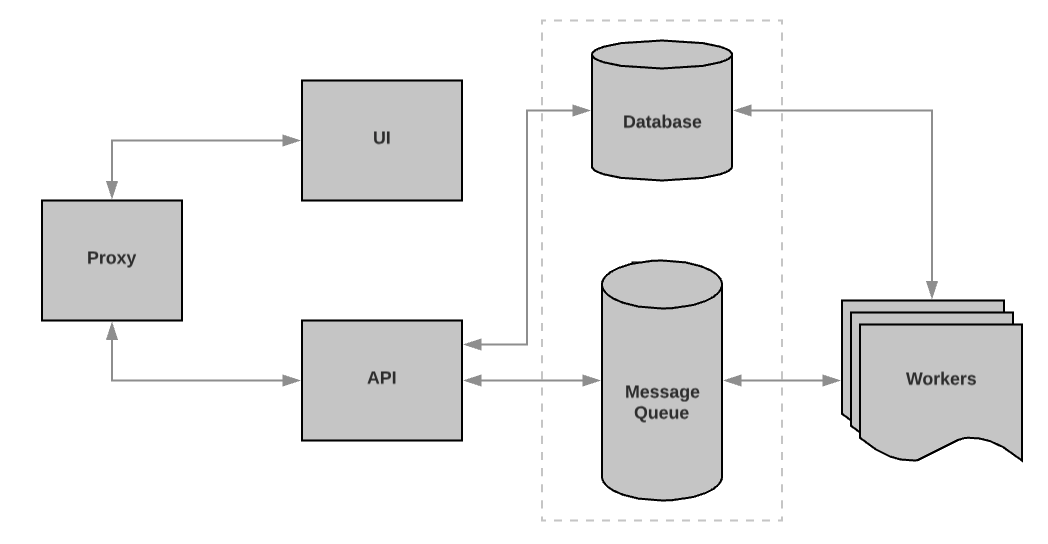
\includegraphics[width=0.5\paperwidth]{Figures/ATHENA_deploy_stack}
\decoRule
\caption[ATHENA Deployment Stack]{ATHENA One Logical Deployment Stack}
\label{fig:deployStack}
\end{figure}

Contrary to typical lab or experimental setup that use for benchmarking or comparison purpose, the ATHENA deployment is, somewhat, in a real world setting and live deployments where users are actively using the system. The development and integral releases are pushing into the deployed sites regularly. Therefore, the deployment and operation consideration mainly favour stable steps and reliable approaches. Deployments are regularly snapshot and backed up. The server instance decommissioning are carefully planned and recycled when the machine vertical scaling is needed to replace the already provisioned environment. 

%\section{Infrastructure}
\noindent \textbf{Infrastructure:} \quad The Australian National eResearch Collaboration Tools and Resources (NeCTAR) is the federally funded research cloud platform where the underlying datacenters span across Australia capital cities. At present, it supports 6000+ virtual machines using around 30,000+\footnote{\url{https://status.rc.nectar.org.au/growth/infrastructure/}} vCPUs across Australia.

ATHENA uses NeCTAR as the main IaaS Cloud provider. NeCTAR infrastructure is implemented and managed using the OpenStack cloud computing framework. The ATHENA deployment is leveraging across two tenancies with total number of 300 vCPU cores allocated for the project. The typical choice of instance size is between \textbf{m1} and \textbf{m2} flavours of \textbf{large}, \textbf{xlarge} \footnote{\url{https://support.ehelp.edu.au/support/solutions/articles/6000055380-resources-available-to-you}} ranging between 4 cores to 16 cores. The choice of base image is \textit{NeCTAR Ubuntu 16.04 LTS (Xenial) amd64}.

The ATHENA source code version control is hosted on Microsoft Visual Studio Team Services (VSTS)\footnote{\url{https://www.visualstudio.com/team-services}}. The deployment is mainly driven by Git Workflow\footnote{\url{https://git-scm.com/book/en/v2/Git-Branching-Branching-Workflows}} and VSTS's build and release pipelines. The VSTS's \textbf{Continuous Integration} (CI) and \textbf{Continuous Delivery} (CD) \parencite{httermann2012devops} are setup to push to the target deployment environments. The terms \textbf{DEV}, \textbf{STAGING} and \textbf{PROD} in Figure~\ref{fig:deployVSTS} represent the development, staging and production deployment environments of the ATHENA software stack. Build-agents are the VSTS build slaves for compiling and building the ATHENA artifacts.

\begin{figure}[H]
\centering
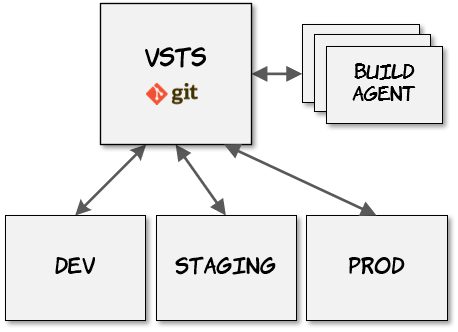
\includegraphics[width=0.3\paperwidth]{Figures/ATHENA_deploy_vsts}
\decoRule
\caption[ATHENA VSTS and Git]{ATHENA VSTS and Git Driven Deployment}
\label{fig:deployVSTS}
\end{figure}

\section{Dockerised Deployment and Scaling}

Initially, the ATHENA stack was deployed in a good old-way of using distro packaging tool \verb|apt-get| and running using \verb|systemd/init.d| daemon services. This has performed through SSH terminal session on the node, e.g:

\begin{small}
\begin{lcverbatim}
apt install mongo
systemctl start mongod
\end{lcverbatim}
\end{small}

\noindent \textbf{IaC Automation Tool:} \quad Nonetheless, this were later change to use Ansible\footnote{\url{https://www.ansible.com}} as IaC automation tool. This improve the scripted knowledge of what has made changes to the server over the system deployment life cycle. The Ansible Playbook scripts were written according to server role such as \verb|db-server.yaml|, \verb|api-server.yaml|, so on. The pros of Ansible are agentless and, its only dependency is SSH which comes in default with most Linux distribution. The cons side of Ansible is that it requires a bit more care to script it in idempotent way. Otherwise the side-effect is detrimental e.g the use of the following task would wipe \verb|vdd| block device each time Ansible script run.

\begin{small}
\begin{lcverbatim}
shell (or command): mkfs.xfs -f /dev/vdd
\end{lcverbatim}
\end{small}
 
For a quick comparison, Chef\footnote{\url{https://www.chef.io}} and SaltStack\footnote{\url{https://saltstack.com}} tools were evaluated as Ansible alternative. The SaltStack can operate in both agent and non-agent mode -- whereas in agentless, it operates as light weight as Ansible. Chef requires an agent to be installed on all the nodes in the cluster fleet which is an overhead. On the other hand, Chef gives the most controlled environment such as retaining the guarantee system state. A more in depth comparison is off interest for this paper, but the next contender would be SaltStack. The justification is solely based in favour of the KISS principle -- \textit{\textbf{K}eep \textbf{I}t \textbf{S}imple and \textbf{S}traightforward}.

\noindent \textbf{Vertical Scaling Issue:} \quad Furthermore, in the beginning, the whole ATHENA stack Figure~\ref{fig:deployStack} was deployed onto the single environment i.e. one VM instance. The pros with this approach is almost zero network latency among software components communication. But it needs a powerful machine. The highest flavour we can request on NeCTAR is \textit{m1.xxlarge: 16 cores, 64GB RAM}, although the real-world experience shows that this is somewhat difficult to get allocation from NeCTAR, which is understandable for a shared research facility. Most importantly, this approach has the potential vertical scaling limit as if requires more resources in one box.

\noindent \textbf{Stateful and Stateless:} \quad The first step of scale out approach is to identify the State nature of the software stack and split between stateful and stateless components. In addition, the components are built into the docker images (i.e. dockerised) and run as containers. Figure~\ref{fig:deployDockerised} depicts the arrangement of this approach -- stateful database containers on \verb|db-server1| node and, pseudo-stateless API, stateless UI and Worker containers on another node. The scaling is a bit easier now. However, this is still a single node container scaling for the worker's Bag-of-Tasks remote job execution discussed in Chapter \ref{Chapter2}.

\begin{small}
\begin{lcverbatim}
docker-compose -f docker-compose.yaml -f staging.yaml  --project-name=stg \
   --scale worker=2
\end{lcverbatim}
\end{small}

\begin{figure}[H]
\centering
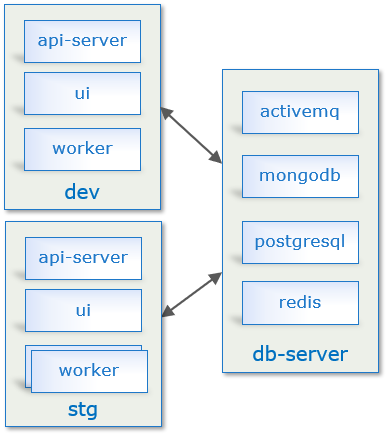
\includegraphics[width=0.4\textwidth]{Figures/ATHENA_dockerize}
\decoRule
\caption[ATHENA Dockerised]{ATHENA Dockerised and split by stateful and stateless components on different nodes}
\label{fig:deployDockerised}
\end{figure}

\noindent \textbf{Dedicated Workers:} \quad As discussed in Chapter \ref{Chapter2}, the worker Remote Job Execution and computation can become very CPU intensive when \textbf{Optimisation algorithms} are activated in the simulated scenario. Further attempt to improve worker's computation throughput, we can split the worker containers into the pool of worker nodes as shown in Figure~\ref{fig:dedicatedWorkers}. This solution is expensive but a good compromise if dedicated worker service is needed for QoS purpose.

\begin{figure}[H]
\centering
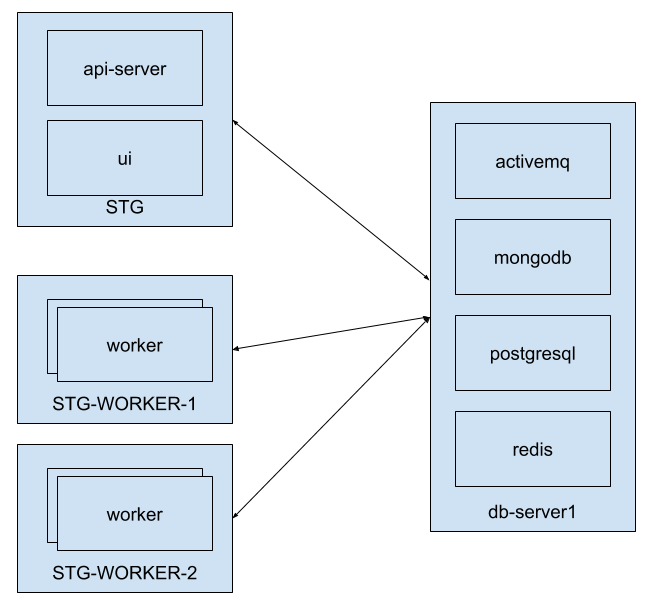
\includegraphics[width=0.4\textwidth]{Figures/ATHENA_dedicated_workers}
\decoRule
\caption[ATHENA Dedicated Workers]{ATHENA dedicated workers on different nodes to form pool of workers}
\label{fig:dedicatedWorkers}
\end{figure}

In fact, this dedicated workers approach is the recommended for Production deployment in the ATHENA deployment guide v1.0\parencite{athenaAllDoc}. It requires network and resources provisions as shown in Figure~\ref{fig:deployNetwork}. 

Note that, only ports 80 and 443 are exposed through the proxy-server to the external (public) network. The rest of the system resources form a trusted private network (subnet) among themselves and is protected behind the firewall for all the ingress network traffic. The private network 10.1.0.0/16 has setup and, a fixed static IP addressing is configured on each of the host systems. The host systems may have 2 NICs (network interface cards) typically eth0, eth1 and have chosen 1 NIC for connecting this private internal network. The recommended network is Gigabit Ethernet (1GbE) or higher speed inter-network connection is assumed.

\begin{figure}[H]
\centering
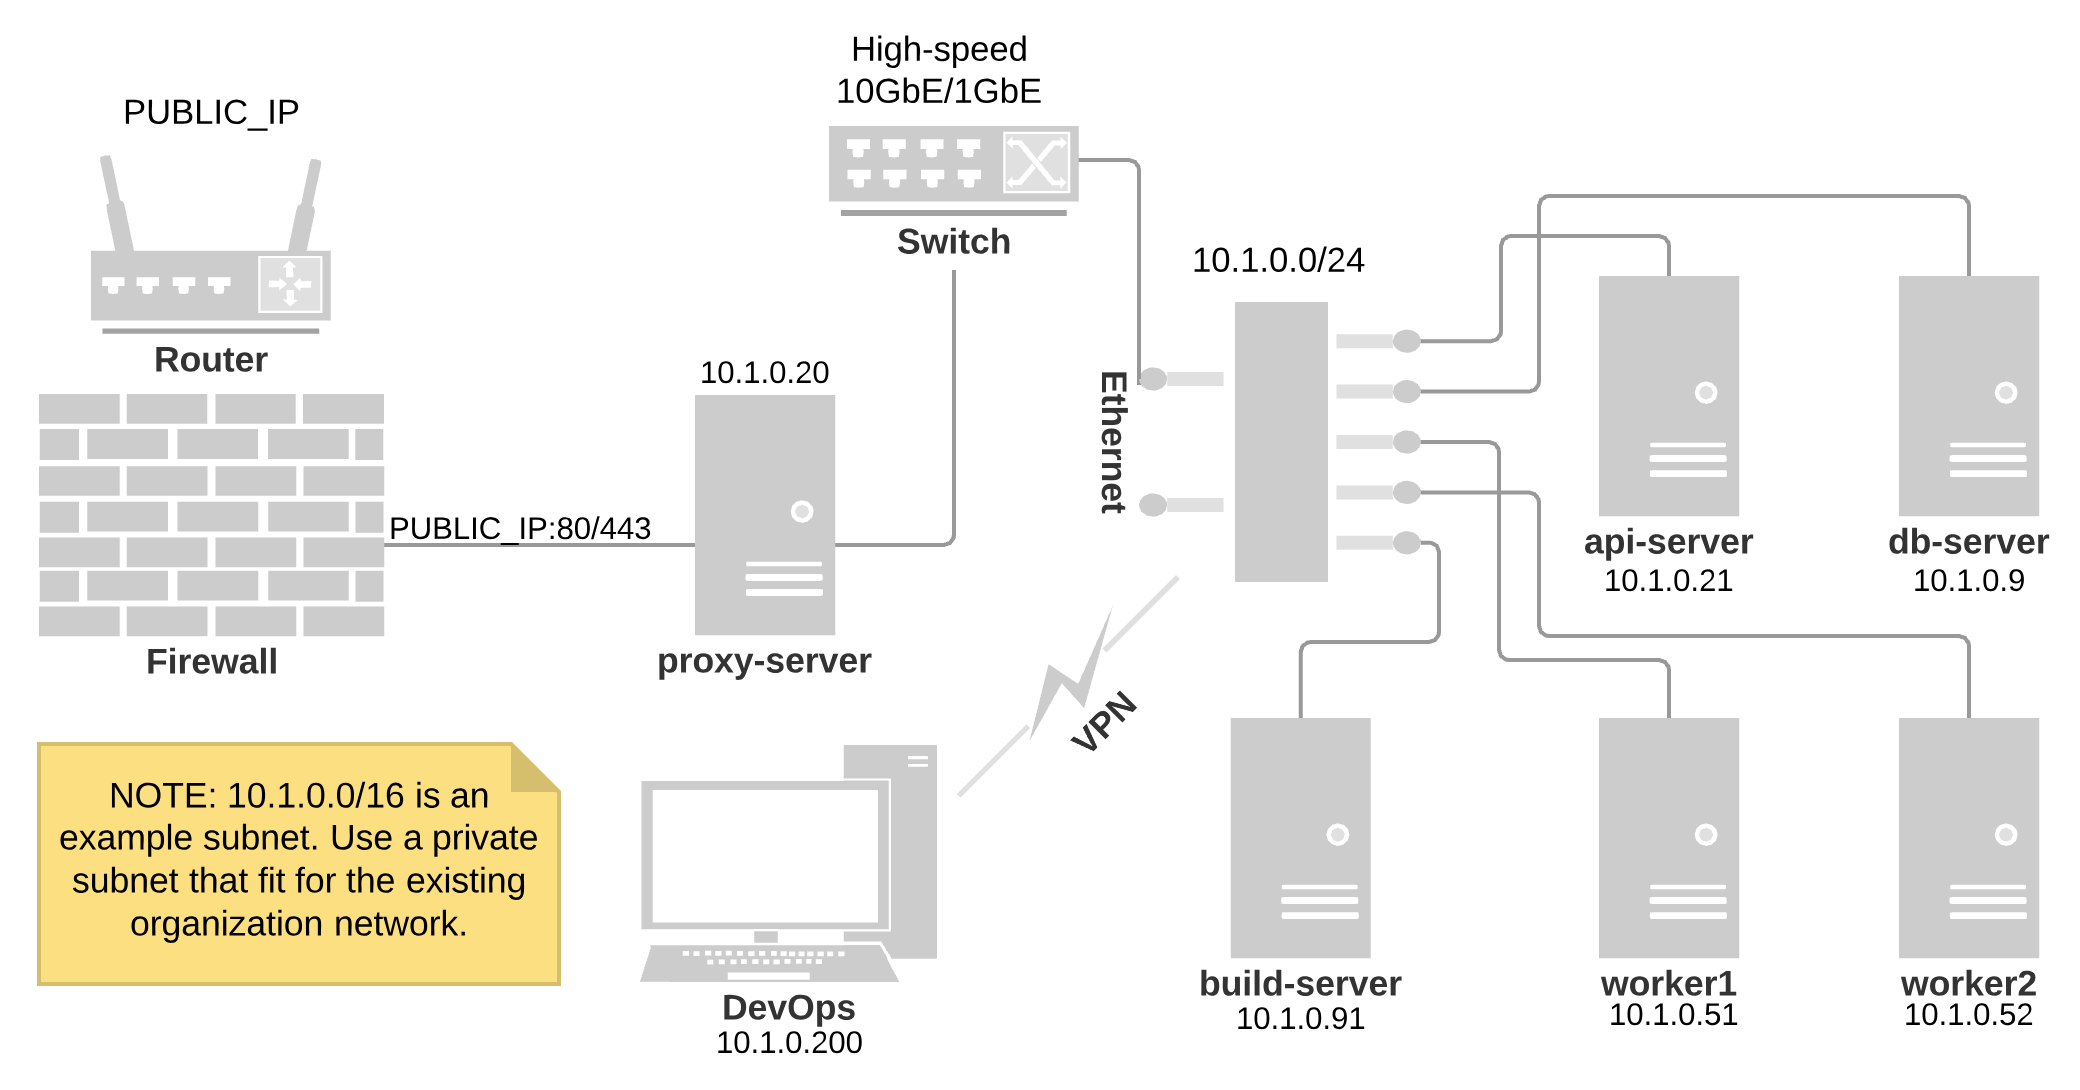
\includegraphics[width=0.7\paperwidth]{Figures/ATHENA_deploy_network_diagram}
\decoRule
\caption[ATHENA Network Diagram]{ATHENA Network Diagram}
\label{fig:deployNetwork}
\end{figure}

In this arrangement, we can horizontally scale out the system well. We can add more database nodes for MongoDB Sharding and Replication\footnote{\url{https://docs.mongodb.com/manual/}} to handle the terabytes (TB) of simulation data and, to retain these simulation data in the system for operational need. We can add more worker nodes into the dedicated worker pool for higher throughput. In ATHENA version 1.0, the api-server is still pseudo-stateless, in such that the Aggregator component as shown in Figure~\ref{fig:conceptArch} is required to aggregate all the results from the simulators computation. This has a potential bottleneck on the api-server. There is a plan to decompose the Aggregator component in a future ATHENA releases.

\section{Docker SWARM Mode}

To this point, we have identified how we can scale the ATHENA system at different layers. However, the system operator still requires to configure and manage these computing resources manually. A good estimated time to add a new worker with the prepared IaC automation scripts; plus NeCTAR VM instance spin up time takes around 20 to 30 minutes. And the operator will have to spin down the instances where there no need of computation demands and keep the system in minimal operational state. This entails the need for self-managed Autonomic Computing \parencite{1160055} and the notion of autonomous cluster management and job execution platform from a pool of computing resources -- also refer as \textbf{Orchestrations} in more recent deployment literature.

Since we have dockerised the entire ATHENA software components, the next best thing is to switch into Docker SWARM mode. Turning into the docker swarm mode is relatively straight forward. On the chosen node, initialize the manager (master) and add (swarm) worker nodes to form Docker swarm cluster. Service scaling is easy, however, the scaling instruction need to manually set it on the swarm manager node through CLI or docker-compose stack deployment \verb|service.[srv_name].deploy.replicas:5| nomenclature.
\begin{small}
\begin{lcverbatim}
docker swarm init --advertise-addr 192.168.99.100
docker swarm join --token SWMTKN-1-[tonken-scrap] 192.168.99.201:2377
docker swarm join --token SWMTKN-1-[tonken-scrap] 192.168.99.202:2377
docker node ls
ID                            HOSTNAME         STATUS          AVAILABILITY
[nxor..] *   swarm-master        Ready          Active          Leader
[ke35...]    swarm-worker1       Ready          Active
[u2wx...]    swarm-worker2       Ready          Active
docker service scale athena_worker=5
athena_worker scaled to 5
\end{lcverbatim}
\end{small}

For the intreset of the thesis length, the details review of how Docker SWARM works\footnote{\url{https://docs.docker.com/engine/swarm/how-swarm-mode-works/nodes/}} is left to its documentation. This thesis takes advantage of the related studies made within the \textit{\groupname}, of which studies \parencite{swarmKubeBench2} benchmarks on the performance and qualitative comparison of Docker SWARM and Kubernetes. There are also vest amount of internet articles available on qualitative comparison e.g. Platform9\footnote{\url{https://platform9.com/blog/kubernetes-docker-swarm-compared/}}. Base on these literatures, we can conclude that the technical merit of both systems is closely matched, however, in the context of the research presenting in this paper, the \emph{built-in Auto-Scaling feature} in Kubernetes has ruled out for a probable auto-scaling solution for the ATHENA system. The justification to \emph{why Kubernetes} decision is somewhat empirical and pragmatic observation over adoption of Kubernetes trend by many Cloud providers and key players, e.g. Google, IBM, Azure, AWS, RedHat to name few. The Chapter \ref{Chapter4} reinforces this hypothesis.

% \parencite{swarmKubeBench}